\begin{bibunit}
\thispagestyle{plain}

\section*{Abstract}
A rigorous check is a significant phase in the design process of control programs of safety-critical cyber-physical systems. Here, we consider such programs to be implemented using IEC~61499 standard for industrial automation. After the check is performed (for example, using formal verification), the engineer needs to ensure that even in unexpected situations, the system will not fail during the runtime, and for this online verification methods can be utilized.

In this work, we consider attaching monitors implemented as basic function blocks to the interface of the controller, thus having a property being monitored represented in the form of a state machine. Now, monitors make the system safer only if their quality is also ensured. Since their complexity is far lower than the complexity of the controller, they can be model checked, however, in the case of IEC~61499 function blocks, open-loop model checking will produce spurious counterexamples as it will allow combinations that are not possible according to the IEC~61499 function blocks semantics (e.g., data transferred without firing the event). The current work addresses this issue and proposes a method for close-loop model checking of monitors, using the non-deterministic twin of a controller under supervision. We present our approach using the system of two orthogonal pneumatic cylinders.

\section{Introduction}
Safety-critical cyber-physical systems must always comply with their requirements before they become operational. One of the important parts of the process of ensuring compliance is checking whether the control program (or controller) of such a system works as expected. This can be done using verification or validation approaches, which are united by the fact that none of them has a hundred percent coverage when dealing with complex industrial-sized systems. In the case of conventional testing or simulation, even if they are automated, some operational environment-related events might be left out and the industrial-sized system might be too complex to have all the possible test cases generated. Formal verification techniques allow the engineer to check the whole state space of the system; however, they suffer from a state-space explosion problem and of being computationally demanding overall when verifying complex systems. To combat this issue, various model abstraction techniques were developed to decrease model complexity (for example, to verify some particular functionality)~\cite{clarke2000,burch1992symbolic}. Another approach is bounded model checking, in which the executions of particular lengths are checked~\cite{biere2003bounded}. This, in turn, brings us back to the problem of missing a longer scenario that leads to failure.

Nevertheless, both approaches avail in finding the issues in the pre-operational stage, and what has to be added is an entity that would observe whether the particular property of the system holds during the runtime and communicate to an error handling system if the malfunction occurs. Such entities are called monitors or observers~\cite{17jhunjhunwala2022monitoring}. They can be internal or external to the system and perform the \emph{online verification}. Online verification has another advantage, i.e., if the changes have to be applied to the control program fast and there is a lack of resources to perform the global re-check, observers will maintain the safety state of the system by communicating the critical errors during the runtime.

In this work, our control programs are implemented following the IEC~61499 standard for industrial automation, and we consider internal monitors represented with basic function blocks, meaning that the properties of the system to be monitored are expressed as individual finite-state machines. This makes our monitors a better target for formal verification, and model checking, in particular, than the control program as a whole, since checking their whole state space requires less computational resources.

Model checking~\cite{clarke1999} is an approach for formal verification, where the formal model of the system is checked during the pre-operational stage, which is called \emph{offline verification}. In addition to a formal model of the system, model checking requires a formal representation of the properties of the system (for example, using linear temporal logic~(LTL)) as input. The model checker then derives all possible execution scenarios and produces counterexamples if the requirements do not hold. The counterexample for a requirement is such an execution scenario (or a system trace) where the requirement fails. 

Now, we propose to perform an offline verification (model checking) over the functional unit developed for online verification. Here, we face the issue that the traditional open-loop approach for model checking will produce spurious counterexamples due to the semantics of IEC~61499 function blocks~(FBs), where, for example, data cannot be sent or received without corresponding events being fired. 
We address this by modeling a non-deterministic twin of the controller and verifying a closed-loop model instead. We demonstrate our approach on a run-through example of two orthogonal pneumatic cylinders moving forward and backward. For model checking, we use NuSMV verifier~\cite{nusmv} and translate our FBs to its programming language (SMV) using the FB2SMV tool~\cite{drozdov2015fb2smv}.

The remainder of this paper is structured as follows. Section~\ref{sec:prelim} gives an overview of IEC~61499 standard and the verification methods of FBDs implemented according to it. Section~\ref{sec:method} describes a methodology for designing a supervised system, which is described in detail on a run-through example in Section~\ref{sec:methodappl}. Section~\ref{sec:concl} concludes the paper.

\section{Preliminaries}
\label{sec:prelim}
\subsection{IEC~61499}
IEC~61499 defines a design paradigm for distributed automation and control systems. The systems are implemented using the graphical language of function block diagrams~(FBDs). An FBD is a set of various interconnected FBs that can be of a basic, complex, or service interface type. In this work, we do not consider the latter. All FBs have their data and event input and output interfaces. The bricks of an FBD are basic FBs that represent atomic functional units. The logic of a basic FB is defined by an execution control chart~(ECC), which essentially is a Moore state machine and consists of states, transitions, and actions. In each state, an algorithm can be executed and/or an event (defined in the output interface of the FB) emitted. Complex FBs are nets of interconnected FBs of any type. The final FBD is assembled using the available FBs.

IEC~61499 systems are event-driven, unlike, for example, \mbox{IEC~61131-3}~\cite{tiegelkamp1995iec} systems that follow a cyclic execution pattern and \emph{event} is a key concept for the standard. Any event input or output can be bound to a subset of data inputs or outputs, respectively, which means that the corresponding data will be received and processed or sent only if the particular event fires. Intuitively, any update of the event variable opens the gates for the data connected to it.

In this paper, we create our observers using basic FBs, incorporating the logic of the condition to be monitored in their ECCs. As in~\cite{toolchain}, we use Non-Deterministic Transitions~(NDT) to create a non-deterministic twin of the controller of two pneumatic cylinders to verify the observers in a closed loop.

\subsection{IEC~61499 verification}
There exists a sufficient amount of literature on the topics of online (dynamic) and offline (static) verification of IEC~61499 FBDs. 

An overview of both static and dynamic verification approaches is given in~\cite{15blech2016comparison}.
\cite{12yoong2010verifying} proposes an approach of converting IEC~61499 FBs to Esterel and its subsequent verification.
In \cite{13yoong2015verification,14bhatti2011observer}, the monitors expressed as IEC~61499 FBs are added not for run-time verification but to better understand the counterexamples produced by the static verification approach. The system represented as a Kripke structure, together with observers and (possibly) computation tree logic~(CTL) formula are provided as input to the verification module. The authors suggest that, if the counterexample is received, the debugging process is simplified, as observers are inserted into the system structure.
\cite{11lindgren2016contract} considers static verification by enriching FBs with formal contracts and addressing verification on the component, algorithm, and ECC levels. In the works~\cite{agn_case_study} and~\cite{agnostic} the authors translate FBDs to SMV closed-loop formal models, \cite{toolchain} continues in this direction and presents a notation within IEC~61499 syntax for the subsequent generation of closed-loop formal models of FBDs and their verification by means of NuSMV. 

Examples of dynamic verification include, for example, \cite{1falcone2022runtime} that proposes adding enforcers to the application, which will not only monitor but adjust the supervised values in case of the property failure to ensure that the correct values are emitted by the controller. In~\cite{3do2020towards, 8ng2019contract}, the authors add assume and guarantee contracts in the form of FBs to the application to monitor the system during the run-time. \cite{4wenger15behavior} introduces behavioral runtime monitors into the 4DIAC framework. These monitors are generated automatically using service sequences extended with behavioral types. Combining various control and verification techniques, a reconfiguration architecture for fault handling in industrial systems is designed in~\cite{10leitao2020fault}. 

Approaches for dynamic and static verification, both, have their advantages and serve their purposes, hence, probably, the best way to ensure the system's correctness is to complement one with the other. However, despite the fact that there are numerous approaches for online verification, very few articles mention that the diagnosis units themselves must undergo a sanity check, which is especially important in relation to IEC~61499 FBs, where an occasional missing event in a transition condition can make a monitor erroneous. The point is outlined in~\cite{9wiesmayr2022supporting} and in~\cite{17jhunjhunwala2022monitoring} an approach to verify the monitors using Timed Net Condition-Event Systems was mentioned. We continue the work~\cite{17jhunjhunwala2022monitoring} and elaborate on the static verification of monitors expressed as IEC~61499 FBs and the challenges it brings. 

\begin{figure*}[htb]
    \centering
    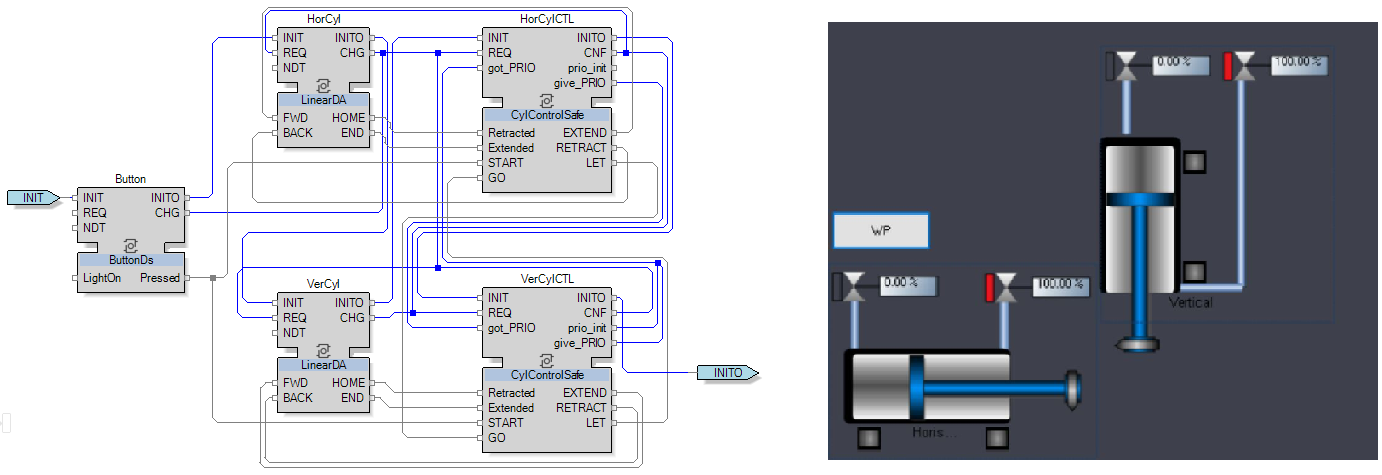
\includegraphics[width=0.98\textwidth]{MX_Papers/Paper3/pic/wholesystem_withhmi.png}
    \caption{The system of two pneumatic orthogonal cylinders. \texttt{HorCyl} and \texttt{VerCyl} simulate the plant (horizontal and vertical cylinder correspondingly), while \texttt{HorCylCTL} and \texttt{VerCylCTL} compose a control program. On the right, the HMI of the system is shown with the situation that should be avoided~-- a simultaneous extension of two cylinders.}
    \label{system}
\end{figure*}

\section{Design methodology for a monitored control program}
\label{sec:method}

For an automation system to function according to its specification, it must be checked using offline verification methods and equipped with online verification mechanisms to ensure that the requirements hold in unexpected circumstances. For this, the runtime verification means should also be checked.
Thus, in this paper, we propose a design methodology for the control programs implemented in form of IEC~61499 FBDs with internal observers (or monitors) that solves the aforementioned problem. Given a plant model (plant simulation program), for a single monitor, the methodology involves the following steps:
\begin{enumerate}
    \item Implementation of the control program.
    \item Verification of the control program in a closed loop with the plant model provided. Depending on its size, the plant model can be simplified and the heuristics for reducing the resulting closed-loop formal model state space may be applied. If the issues are found, the engineer has to address them and repeat this step until the verification result is positive.
    \item Formulation of a desired property to be observed in the form of a finite state machine and its implementation as a basic FB, i.e., implementation of the monitor.
    \item Implementation of the simplified non-deterministic twin of the controller that can produce any combination of outputs based on any combination of inputs. Verification of the created monitor in a closed loop with the twin. The properties to be formulated for the verification procedure, intuitively, are the following: the monitor indicates a failure when the failure occurs and the monitor does not report a failure when the controller functions as expected. If problems are found, they should be eliminated, and the system re-checked. This step should be repeated until the verification yields no counterexamples.
    \item Verification of the monitor in a closed loop together with the real control program.
    \item Verification of the monitor in a closed loop together with the control program where the fault was injected. Steps~5 and~6 may employ bounded model checking techniques or heuristics for state space reduction. The steps must be repeated if there were found issues to be addressed.
\end{enumerate}

The main contribution is concentrated in step~4.
In the next sections, we demonstrate our methodology step by step on a run-through example of a system of two pneumatic cylinders, especially focusing on step~4.

\section{Methodology application}
\label{sec:methodappl}
\subsection{Steps 1 and 2: control program implementation and verification}

Our task was to create a control program for two orthogonal pneumatic cylinders that move towards each other and back by pressing a switch button. The plant simulation model was implemented as an IEC~61499 FBD in EcoStruxure Automation Expert (EAE).

The aim of the controller was to allow both cylinders to extend and retract once the button was pressed. The following safety requirement was to prevent the cylinders from colliding.
Thus, we implemented the priority system so that the horizontal cylinder can start moving only when the vertical cylinder is retracted. The complete system is presented in Figure~\ref{system}. Here, the control program consists of two controllers (for vertical and horizontal cylinders) of the same FB type that are connected in a closed loop with their plant models (cylinders). When the button is pressed, the command \texttt{START} is sent to the controllers and the cylinder with the higher priority gets the command to start its moving cycle (extend and retract). After the controller recognizes that its cylinder is retracted, it sends the priority giving event (\texttt{give\_PRIO}) to the vertical cylinder and sets the variable \texttt{LET} to true, allowing the vertical cylinder to take its turn.

In our case, the system is of a moderate size and we can apply model checking as is, without abstracting the system or using bounded model checking.
Thus, we translated our system to SMV code using the FB2SMV tool and checked the following LTL formula with NuSMV verifier: \texttt{G $\neg$(Ver.EXTEND $\land$ Hor.EXTEND)} (where \texttt{Ver} and \texttt{Hor} are \texttt{VerCylCTL} and \texttt{HorCylCTL} correspondingly), 
which means that at every discrete time step, the two cylinders never get the command to extend simultaneously. The verification result was successful. 

\subsection{Step 3: Monitor implementation as a basic FB}

The next step was to create a monitor that would observe whether the safety property (i.e., two cylinders should never receive the command to extend simultaneously) is maintained by the system during the runtime. We implemented the monitor as a basic FB and assumed that it would be connected to the controllers as in Figure~\ref{fig:monitorplacement} (other connections are not depicted for the sake of clarity).

\begin{figure}[h!]
    \centering
    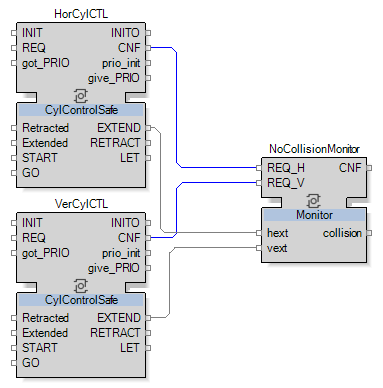
\includegraphics[width=0.35\textwidth]{MX_Papers/Paper3/pic/monitorplacement.png}
    \caption{Monitor \texttt{NoCollisionMonitor} connected to the controllers (other connections are not shown for clarity).}
    \label{fig:monitorplacement}
\end{figure}

The monitor receives the \texttt{EXTEND} outputs from both controllers together with their events \texttt{CNF} and communicates whether the collision is occurring by setting its output \texttt{collision} to \texttt{true} and triggering the \texttt{CNF} event. The ECC of the monitor is presented in Figure~\ref{fig:monitorecc}.

\begin{figure}[h!]
    \centering
    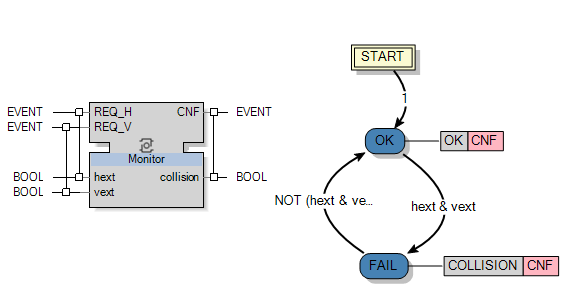
\includegraphics[width=0.48\textwidth]{MX_Papers/Paper3/pic/monitorecc.png}
    \caption{Interface of the monitor and its ECC. Algorithms \texttt{OK} and \texttt{COLLISION} set output variable \texttt{collision} to \texttt{false} and \texttt{true} correspondingly.}
    \label{fig:monitorecc}
\end{figure}

\subsection{Step 4: monitor verification with a non-deterministic twin of the controller }
\label{sec:monitorver}
The next step is to verify the implemented monitor in a closed loop with the controller (which we decompose into two controllers~-- for vertical and horizontal cylinders). In our case, the controllers are represented with basic FBs, and the closed-loop model checking will produce the result within an acceptable time interval. However, we will have to close the loop on the inputs of the controllers as well, meaning that we will either have to model simplified plants or provide other means for the controllers to produce all the possible combinations of their output values. Moreover, even if we succeed in closing the loop on the controllers, in case issues are found during the model checking, counterexamples will be hard to decipher as they will elongate and dozens of additional variables will be added to the system state.

Thus, we propose creating a \emph{non-deterministic twin} of the controller, which will be represented with two FBs of the same type just like our individual cylinder controllers. Now, let us disclose the notion of a non-deterministic twin~(ND twin). 

To model check the monitor, it is important that the model checker would infer all the possible combinations of its inputs, meanwhile triggering the events associated with them. Therefore, the goal of an ND twin is to abstract the logic of the controller by saving its key states, where the variables that are monitored change and add the non-deterministic transitions~(NDT) between them. Such events in an FBD turn into non-deterministic inputs in the SMV module of the corresponding FB, generated by FB2SMV as described in~\cite{agn_case_study}. 

The ECC of our individual controller of the cylinder together with its ND twin are presented in Figure~\ref{fig:ndtwinecc}. Two states that change the supervised variable \texttt{EXTEND} are \texttt{EXT}, \texttt{RETRACT}, and \texttt{STOP}. We kept them in the ND~twin and added NDTs between them so that at any time any output could be produced. From the algorithms, we remove everything that does not influence the variable \texttt{EXTEND} and leave only the \texttt{CNF} event associated with it. Figure~\ref{fig:ndtwinloop} shows two ND~twins of the controllers connected to our monitor.

\begin{figure}[t]
    \centering
    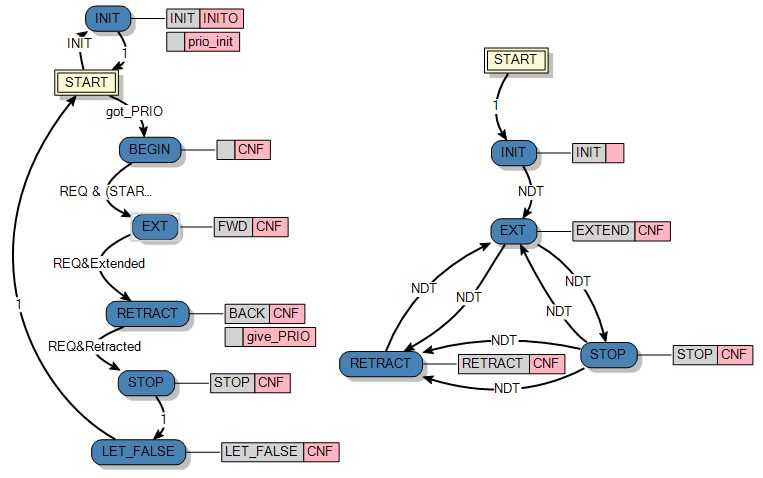
\includegraphics[width=0.5\textwidth]{MX_Papers/Paper3/pic/ndtcontrollereccs.png}
    \caption{ECCs of the cylinder controller (to the left) on of its ND~twin (to the right).}
    \label{fig:ndtwinecc}
\end{figure}

\begin{figure}[b]
    \centering
    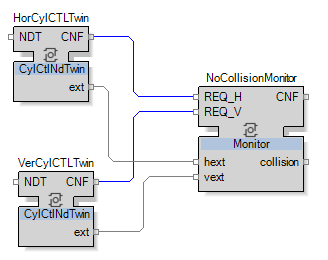
\includegraphics[width=0.34\textwidth]{MX_Papers/Paper3/pic/ndtwinloop.png}
    \caption{Connection of the monitor to ND~twins of the cylinder controllers.}
    \label{fig:ndtwinloop}
\end{figure}

When the system is converted to SMV, the first step is to verify that we can indeed get all the values of the monitor input, that is, our ND twins function according to their specifications. The set of properties that make up the specification can be created according to the following template. 

Assume that we have a set of all the supervised variables in a single ND~twin $U$.
$\forall u \in U, \exists D_u$, where $D_u$ is a domain of $u$. Then, $\forall u \in U, \exists V_u = \{(u,v) \:|\: v \in D_u\}$, where $V_u$ a set of all possible assignments of $u$. Now, a set of all the possible combinations of the variables values is $C = V_{u_1}\times\ldots\times V_{u_n}, n = |U|$. Having $C$, we can now formulate the CTL specifications to be checked as a set $S$:
$$S = \{\textbf{AG} \:\neg(\bigwedge_{p \in P} u(p) = v(p)) \:|\: P \in C\},$$
where $P$ a set of variable and value pairs, $u(p)$ returns the variable name of pair $p$ and $v(p)$ its value. Thus, if any of the specifications from $S$ are satisfied, it means that their corresponding combination cannot be generated by a formal model of an ND~twin.
Similarly, we check if the observer can get all the possible combinations of input values.

In our case, we checked the following specifications for the ND~twins (here, \emph{twin} is replaced with the corresponding names of the FBs for horizontal and vertical cylinders controllers twins): \texttt{AG twin.EXTEND} and \texttt{AG $\neg$twin.EXTEND},~-- and four specifications for the monitor of type \texttt{AG $\neg$(NoCollisionMonitor.hext $\land$ NoCollisionMonitor.vext)} (we omit others to save space). All the specifications failed, which means that all the combinations were possible in our model. 

Now, that we know that our model produces all the combinations of inputs, we can formulate the properties of the monitor to be checked. The first one tells that whenever the monitor gets the signals that both of the cylinders extend simultaneously, it produces the warning. Its LTL equivalent is: \texttt{\textbf{G} ((m.hext $\land$ m.vext) $\rightarrow$ (m.hext $\land$ m.vext \textbf{U} m.collision))}, where \texttt{m.} is short for \texttt{NoCollisionMonitor.}. Here we use operator \textbf{U}~-- ''until'' instead of \textbf{X} (''next'') or no temporal operator due to the specifics of the generated SMV model, where several model evaluations should occur to obtain the result of the FB output.

The second property tells that if the cylinders are not extending simultaneously, the collision is not reported, which is in LTL: \texttt{\textbf{G} ($\neg$(m.hext $\land$ m.vext) $\rightarrow$ \textbf{F} $\neg$ m.collision)}.

Both properties were satisfied by our monitor.

\subsection{Steps 5 and 6: monitor verification with the real and erroneous controller}

Now, we add the monitor to the system and check whether we connected it properly by verifying the system with the monitor as a whole. If the system at step~2 was checked using state-space reduction techniques, they can be applied here as well.

To check whether the monitor works when there is an error in the system, we inject the fault manually. In our case, we remove the priority mechanism from the controllers so that, by pressing the button, both cylinders extend simultaneously. The ECC of the erroneous cylinder controller is shown in Figure~\ref{fig:errctlecc}.

With both systems, we partially verify the same properties as in Section~\ref{sec:monitorver}. In both cases, we check whether all combinations of input values are possible for the monitor. The correct system reports that there is no possibility for two cylinders to get the extension command simultaneously, while only this is possible in the malfunctioned system. Then, we check the monitor properties, i.e., whether it reports the collision when it happens and does not report spurious collisions. Since the collision is not allowed in the first system, we omit the first monitor property, when checking the correct system, similarly, we omit the second property, checking the erroneous one. In both systems the checked properties hold, thus we can conclude that the monitor and its connections are correct.

\begin{figure}[t]
    \centering
    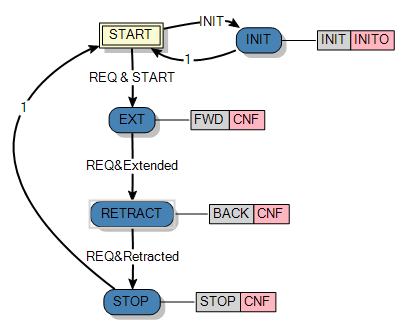
\includegraphics[width=0.34\textwidth]{MX_Papers/Paper3/pic/errctlecc.png}
    \caption{The ECC of the erroneous cylinder controller.}
    \label{fig:errctlecc}
\end{figure}

\section{Conclusion and future work}
\label{sec:concl}

In this paper, we presented a design methodology for the supervised system implemented in form of IEC~61499 FBD, putting special attention to the verification of the supervision mechanisms, that is, the monitors. This methodology allows using formal verification with state-space reduction or abstraction techniques while verifying the system as a whole, while creating reliable means for online observation of its function. Our main contribution is the approach for extensive closed-loop verification of monitors implemented in form of IEC~61499 FBs using the simplified non-deterministic twins of the controllers.

Having the system monitored gives an additional advantage while introducing small changes to the system when, for instance, the time does not permit performing the whole recheck. If the connections to the monitor do not change, with the proper setting of an error handling unit, the system will stay safe even if the new change leads to a failure.

The manual implementation of the proposed methodology may seem to cost time and effort; however, the process can be automated. Our future work in this direction focuses on creating the plugin to an open-source IDE for IEC~61499 programs, FBME~\cite{fbme}, that would implement the algorithm that distinguishes the key states of the controller, which change the variables under supervision, and generate a FB with NDTs between such states (i.e, ND~twin). The properties that should be checked on an SMV model of an ND~twin can also be generated automatically following the definition that we used in the current work. Thus, if we assume such a plugin, the input data for it would be a monitor, a supervised controller, and a set of temporal properties with which the monitor should comply. The subsequent check of the monitor injected into the system as a whole can be done semi-automatically, depending on the size of the SMV model of the system. 

Another direction of future work is to explore the scalability of our monitor-checking approach and verify more complex properties that include not only inputs of the monitors but any variable in the system, as well as monitors and controllers implemented as composite FBs.

\section*{Acknowledgments}

This work was supported, in part, by the HORIZON 2020 project 1-SWARM funded by the European Commission (grant agreement: 871743) and Horizon Europe project Zero-SWARM funded by the European Commission (grant agreement: 101057083).

We also wish to thank Dr. Igor Buzhinsky for suggesting us the missing piece of the puzzle during the work on Section~\ref{sec:monitorver}.

\putbib
\end{bibunit}
